\documentclass{article}
\usepackage{amsmath}
\usepackage{hyperref}
\usepackage{graphicx}
\usepackage{booktabs}
\usepackage{float}
\hypersetup{
	colorlinks=true,
	linkcolor=blue,
	filecolor=magenta,      
	urlcolor=blue,
	pdfpagemode=FullScreen,
}
\usepackage{natbib}
\bibliographystyle{plainnat}

\begin{document}
	
\section{Abstract}

This document aims to do the following:
\begin{itemize}
	\item Establish and test a workflow for SBI optimisation on process equipment
	\item Evaluate its use in identifying sensor and parameter drift
	\item Evaluate the drawbacks and challenges on using SBI on real-data
	\item Compare the advantages of using SBI against other optimisation routines
\end{itemize}

\section{Introduction}

Optimisation and tuning of simulators against real data in the automation sphere can be a challenge. 

\section{Methodology}

\subsection{Development of CSTR Model}
\label{sec:cstr-model}

The same CSTR (Continuous Stirred Tank Reactor) model as developed by \cite{pilario2018canonical} is used in this study. This refers to a reactor with a first order, exothermic reaction with a cooling jacket where the cooling water is regulated by a temperature controller. The full set of differential equations that describe the dynamic process are presented below:

\begin{align}
	\frac{dC}{dt} = Q/V(C-C_i)-kC \\
	\frac{dT}{dt} = (T_i-T)\frac{Q C_p}{V}+\frac{kC\Delta H_{r}}{\rho C_p}-\frac{UA(T-T_c)}{\rho C_p V}\\
	\frac{dT_c}{dt} = (T_{ci}-T_{c})\frac{Q_c}{V_c} +\frac{UA(T-T_c)}{\rho_c C_{pc} V_c	} 
\end{align} 

The reaction is assumed to be an exothermic 1st order reaction that follows the Arrhenius equation for its reaction coefficients:

\begin{equation}
	k = k_0 e^{-E_a/RT}
\end{equation}

The rate of cooling water itself is controlled by the cooling water valve which strives to reach a temperature setpoint. This was implemented using a PI controller. 

\begin{equation}
	Q_c = Q_{c, 0} + K_p(T-T_{sp}) + \frac{1}{\tau_i}\int_{0}^{T}(T-T_{sp})dt 
\end{equation}

The same constants as those used by \cite{pilario2018canonical} are used with the exception of the integral time ($\tau_i$) which was set to 0.5 min$^{-1}$ to enable controller stability. 

The differential equations were solved the \textbf{solve\_ivp} method from "scipy" using the Runge-Kutta (\textbf{RK45}) method. A maximum step size of 0.01 minutes was used to help with solver convergence. The PI controller followed standard implementation. It was set to update the controller value only after an elapsed dt of 0.01 minutes and contains anti-reset windup to avoid integration issues when reaching controller saturation. The model for the baseline case was run for 20 minutes. The full code is available online at X.

\subsection{Simulation of "Real" Process Data}

To generate "process data" from this model, a few things can be done to make it look real. This includes the following:

\begin{itemize}
	\item Dynamic perturbation of the inlet values of $C_i$, $T_i$ and $T_{ci}$
	\item Adding Gaussian white noise to all variables to replicate sensor noise
	\item Introducing stochasticity to the model dynamics
	\item Sensor drift to certain variables (i.e. offsetting the true value by a constant)
	\item Parameter mismatch where key system parameters differ from their "ideal" value
\end{itemize}

The last point is known in the literature as the process-model mismatch and this can be emulated by changing the expected theoretical behaviour of the model or changing the simulation parameters over time.  Several datasets that involve normal operation can be generated by simulating the system for a long time (i.e. 30 days = 43200 minutes). The stochastic perturbations, dynamic change in the simulator parameters and sensor drift that was mentioned in the previous section can be applied to replicate variability of operating conditions. The following changes were performed:

\begin{itemize}
	\item Catalyst decay: $\alpha kC$ where $\alpha=1-0.1 t/T_{crit}$  
	\item Cooling jacket fouling: $\beta \frac{UA(T-T_c)}{\rho C_p V}$ where $\beta=1-0.1 t/T_{crit}$
	\item Dynamic perturbation of inlet conditions every 60 minutes 
	\begin{itemize}
		\item $T_i$ and $T_{ci}$ vary between 348 K and 352 K
		\item $C_i$ varies between 0.9 mol/L and 1 mol/L
	\end{itemize}
	\item Sensor drift where $T$ is incremented by 2 K and $C_i$ is incremented by 0.1 mol/L after simulation
	\item Gaussian noise added to all sensors with an amplitude of 0.5\% of their maximum value after simulation
	\item Gaussian noise added to the differential equations with amplitude of 0.1 mol/L/s for the component balance and 10 K/s for both energy balances
\end{itemize}

$T_{crit}$ for points 1 and 2 above was set to 43200 minutes indicating that the catalyst and cooling jacket effectiveness drops by 10\% after a month.

\subsection{Base Optimisation: Least Squares}

Least squares optimisation is the the default vanilla optimisation routine that can be run. The objective function is defined as the minimisation of the sum of the square of the difference between each parameter and its desired value:

\begin{equation}
	\theta \leftarrow min(\sum_{n=1}^{N}(y_i-\hat{y}_i\vert_\theta)^2)
\end{equation}

where $\theta$ is the parameter array, $N$ is the total number of variables (in this case 3: $C$, $T$ and $T_c$), $y_i$ is the true value of the variable and $\hat{y}_i\vert_\theta$ is the predicted value from the model using parameters $\theta$. Each variable is normalised by its initial value to ensure that all variables have equal weighting in the objective function. The minimisation algorithm is performed using the \textbf{minimize} package \textbf{scipy} as developed by \cite{2020SciPy-NMeth}.	The Nelder-Mead in particulat was used where the the initial parameter values were initialised randomly to avoid local minima.

\subsection{SBI Implementation}

SBI was implemented by using the \textbf{SBI} package in PyPI	as developed by \cite{tejero-cantero2020sbi}. The SNPE (Sequential Neural Posterior Estimation) method was used to perform the likelihood-free inference to estimate the posterior from the simulator. The simulation itself was run by solving the equations specified in Section \ref{sec:cstr-model} for 10 minutes and using the solved values from the last time step as the output. A separate posterior was trained for each set of initial conditions changing only the number of simulations (\textbf{num\_simulations}) hyperparameter for sensitivity studies.

\subsection{Optimisation Workflow}

Two main parameters were optimised in this study: the Arrhenius constant ($k_0$) and the heat transfer efficiency of the cooling jacket ($UA$). The study in this paper is performed as follows:
\begin{itemize}
	\item Optimisation routines were compared against 'clean' simulation data in an attempt to recover the true simulation parameters.
	\item Several SBI models were trained on the 'real-data' in an effort to estimate the parameter and sensor drift in the data over time
	\item SBI model was run on controller saturation data to quantify drawbacks in optimising against real data.
\end{itemize}

The true parameters of the model for the clean simulation data is 7.2e10 min$^{-1}$ and 7e5 cal/min/K for $k_0$ and $UA$ respectively. These are also the initial values of the parameters in the 'real-data' at t=0 before the linear decay of both parameters begins to set in. The PI controller is not part of the CSTR model during optimisation as the flow rate $Q_c$ is known at all times. 


\section{Results}

\subsection{CSTR Model Validation}

The CSTR model defined in Section \ref{sec:cstr-model} was simulated for 20 mins over time with the inlet values of 0.97 mol/L, 351.5 K, 351.6 K, 150 L/min for $C_i$, $T_i$, $T_ci$ and $Q$ respectively. The initial values were set to the same values as the inlet conditions. The results over time for the 4 dynamic variables is presented in Figure \ref{fig:baseline_model_results.png}. It can be seen that the system tends to a steady value within about 20 minutes. The final values for $C$, $T$, $T_c$ and $Q_c$ are 0.1 mol/L, 430 K, 416 K and 147 mol/L respectively which is inline with those recorded by \cite{pilario2018canonical}. A notable caveat is that the integral time in the controller parameters had to be changed to 0.5 min$^{-1}$ to avoid controller instability. This end result is robust to different controller bias and sample times.

\begin{figure}[H]
	\centering
	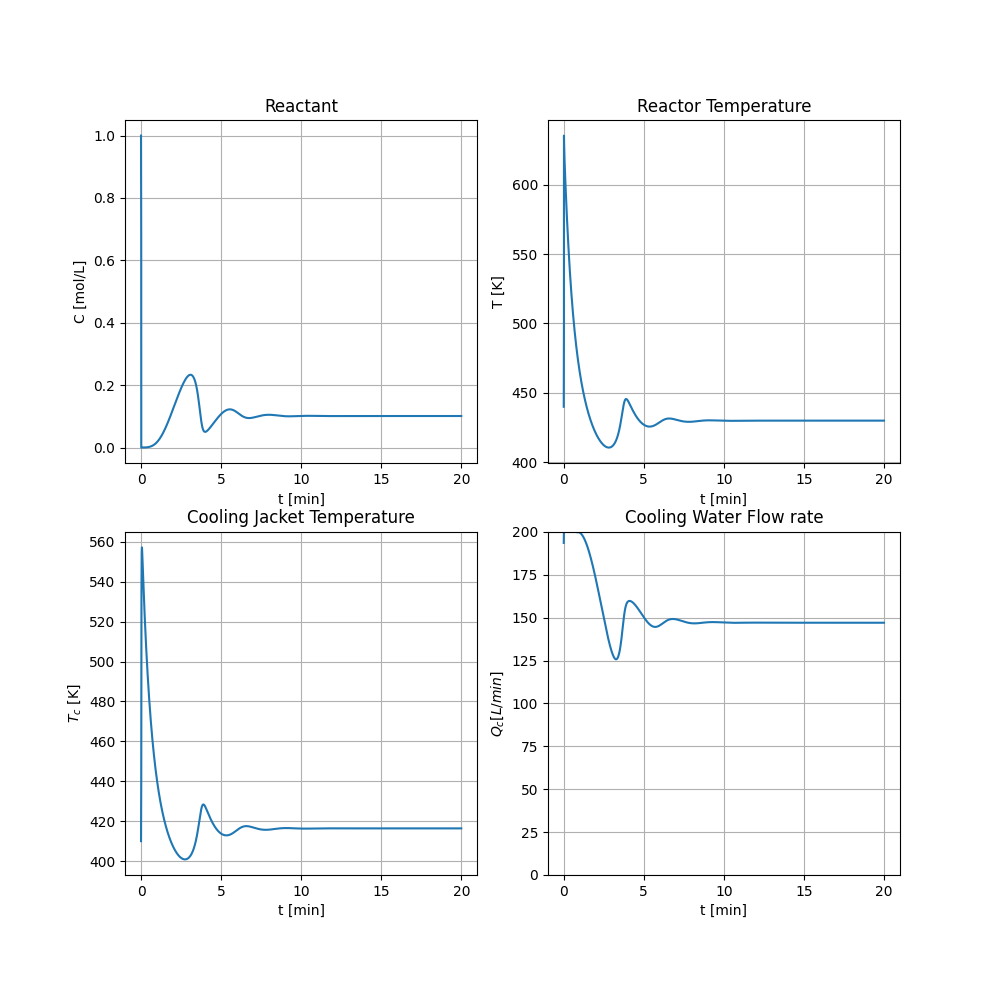
\includegraphics[width=1\textwidth]{img/baseline_model_results}
	\caption{System variables over time}
	\label{fig:baseline_model_results.png}
\end{figure}


\subsection{'Clean' Simulation Data Optimisation}

The CSTR model used for optimisation was modified to no longer use the PID controller, to use the initial conditions of 0.1 mol/L, 430 K, 416 K for $C$, $T$ and $T_c$ respectively and to return the last value of the dynamic variables after 10 minutes which is assumed to be at steady-state. The simulation data that was used for the optimisation was generated by the simulator and was used to test the optimisation routines is 0.11 mol/L, 428.70 K and 415.99	 K for $C$, $T$ and $T_c$ respectively.

The vanilla optimisation method gave the following results:

[insert figure of vanilla optimisation results]

The main hyperparameter of choice for the SBI optimisation was the number of simulations to perform in order to train the neural network. It was found that around 1000 simulations were best/sufficient in retrieving the best estimates of the true parameters. The distribution of the parameters after sampling 10000 times from the posterior is shown in Figure \ref{fig:sbi-clean-sim-data-1000-sims}. Overall, less than 0.5\% of simulations were rejected due to not meeting the local tolerance limits.


\begin{figure}[H]
	\centering
	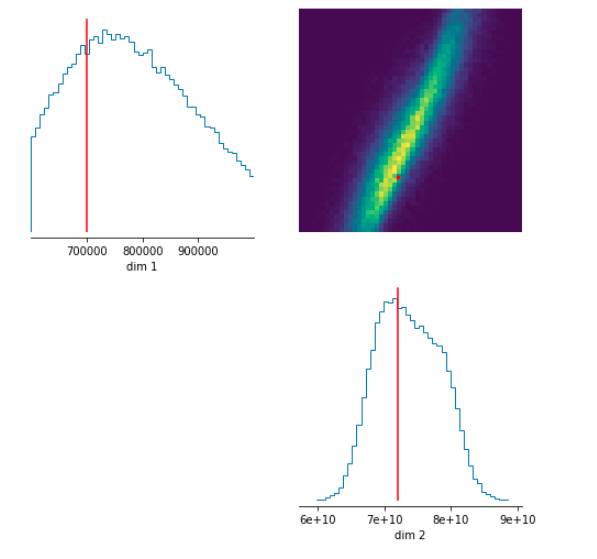
\includegraphics[width=1\textwidth]{img/sbi-clean-sim-data-1000-sims.png}
	\caption{SBI pair plot for the 2 optimisation parameters}
	\label{fig:sbi-clean-sim-data-1000-sims}
\end{figure}

The true parameters were estimated to be 7.8e5 cal/min/K and 7.4e10 min$^{-1}$ for the $UA$ and $k_0$ parameters respectively. These are around 11\% and 2\% off the values of the true parameters which is a significant difference. Furthermore, the distribution is relatively broad with a noticeable likelihood of the solution existing at either end of the parameter limits. This is down to the correlation between the 2 parameters whereby a higher rate constant $k_0$ must translate to a higher value for $UA$ to return the same observation. This because a higher reaction rate causes more heat to be generated from the exothermic reaction and this needs to be additionally removed by improving the rate of heat transfer by the cooling jacket. 



\subsection{Tracking Sensor and Parameter Drift}

\subsection{Controller Saturation}

\bibliography{cstr-sbi}
\end{document}